\chapter{Shape-from-Shading}
\label{ch:sfs}

ASP provides a tool, named \texttt{sfs}, that can improve the level of
detail of DEMs created by ASP or any other source using
\textit{shape-from-shading} (SfS).

The tool takes as input one or more camera images, a DEM at roughly the
same resolution as the images, and returns a refined DEM.

\texttt{sfs} works only with ISIS cub images. It has been tested only
for Lunar LRO NAC datasets. As seen later in the text, it returns reasonable
results as far as $85^\circ$ South on the Moon.

Currently, \texttt{sfs} is computationally expensive, and is practical
only for DEMs of size up to $1000\times 1000$ pixels. It can be very
sensitive to errors in the position and orientation of the cameras, the
accuracy of the initial DEM, and to the value of the smoothing term used
to ensure that the output DEM is not overly noisy.

The \texttt{sfs} program can model position-dependent albedo, different
exposure values for each camera, shadows in the input images, and regions
in the DEM occluded from the Sun. It can refine the positions and orientations
of the cameras, and supports the Lambertian and Lunar-Lambertian reflectance
models.

The tool works by minimizing the cost function
$$
\int\!\! \int \! \sum_k \left[ I_k(\phi)(x, y) - T_k A(x, y)
  R_k(\phi)(x, y) \right]^2\, + \mu
\left\|\nabla^2 \phi(x, y) \right\|^2 \, dx\, dy
$$

Here, $I_k(\phi)(x, y)$ is the $k$-th camera image interpolated at
pixels obtained by projecting into the camera 3D points from the terrain
$\phi(x, y)$, $T_k$ is the $k$-th image exposure, $A(x, y)$ is the
per-pixel albedo, $R_k(\phi)(x, y)$ is the reflectance computed from the
terrain for $k$-th image, $\left\|\nabla^2 \phi \right\|^2 $ is the sum
of squares all second-order partial derivatives of $\phi$, and $\mu > 0$
is a smoothing term. We use either the regular Lambertian reflectance model,
or the Lunar-Lambertian model \cite{mcewen1991photometric}.

Below we show two examples of running \texttt{sfs}, first for one image,
and then for multiple images with bundle-adjustment and modeling the shadow
threshold.

\section{How to get good test imagery}

We obtain the images from
\url{http://wms.lroc.asu.edu/lroc/search} (we search for EDR images of
type NACL and NACR). 

A faster (but not as complete) interface is provided by
\url{http://ode.rsl.wustl.edu/moon/indexproductsearch.aspx}. The related
site
\url{http://ode.rsl.wustl.edu/moon/indextools.aspx?displaypage=lolardr}
can provide LOLA datasets which can be used as ground truth.

We advise the following strategy for picking images. First choose a small
longitude-latidue window in which to perform a search for imagery. Pick
two images that are very close in time and with a big amount of overlap.
Those will create a stereo pair and an initial DEM. Then search for 
other images close to the center of the maximum overlap of the first
two images. Pick one or more of those, ideally with different illumination
conditions than the first two, and run SfS for example with the first
and the third image. 

To locate the area of spatial overlap, the images can be map-projected (either
with \texttt{cam2map} with a coarse resolution) or with \texttt{mappproject}
(using say the LOLA DEM as the terrain to project onto, or the DEM obtained
from running \texttt{stereo} on those images). Then the images can be examined
in \texttt{stereo\_gui} while turning on the mode to render them using their
georeferences.

\section{Running sfs at 1 meter/pixel using a single image}

In both this and the next section we will work with LRO NAC images taken
close to the Lunar South Pole, at $85^\circ$ of latitude (the tool was
tested on equatorial regions as well). We will use four images,
M139939938LE, M139946735RE, M173004270LE, and M122270273LE.

We first retrieve the data sets, convert them to ISIS cubes, initialize
the SPICE kernels, and perform radiometric calibration and echo
correction. Here are the steps, illustrated on the first image:
\begin{verbatim}
  wget http://lroc.sese.asu.edu/data/LRO-L-LROC-2-EDR-V1.0/\
LROLRC_0005/DATA/SCI/2010267/NAC/M139939938LE.IMG
  lronac2isis from = M139939938LE.IMG to = M139939938LE.cub
  spiceinit from = M139939938LE.cub
  lronaccal from = M139939938LE.cub to = M139939938LE.cal.cub
  lronacecho from = M139939938LE.cal.cub to = M139939938LE.cal.echo.cub
\end{verbatim}
We rename, for simplicity, the obtained four processed datasets to
A.cub, B.cub, C.cub, and D.cub.

The first step is to run stereo to create an initial guess DEM. We
picked for this the first two of these images. These form a stereo pair,
that is, they have a reasonable baseline and sufficiently close times of
acquisition (hence very similar illuminations). These conditions are
necessary to obtain a good stereo result.
\begin{verbatim}
parallel_stereo --job-size-w 1024 --job-size-h 1024 A.cub B.cub    \
                --left-image-crop-win 0 7998 2728 2696             \
                --right-image-crop-win 0 9377 2733 2505            \
                --threads 16 --corr-seed-mode 1  --subpixel-mode 3 \
                run_full1/run
\end{verbatim}
Next we create a DEM at 1 meter/pixel, which is about the resolution
of the input images. We use the stereographic projection since this
dataset is very close to the South Pole. Then we crop it to the region
we'd like to do SfS on.
\begin{verbatim}
  point2dem -r moon --stereographic --proj-lon 0 \
    --proj-lat -90 run_full1/run-PC.tif
  gdal_translate -projwin -15471.9 150986 -14986.7 150549  \
    run_full1/run-DEM.tif run_full1/run-crop-DEM.tif
\end{verbatim}
This creates a DEM of size $456 \times 410$ pixels.

Then we run \texttt{sfs}:
\begin{verbatim}
  sfs -i run_full1/run-crop-DEM.tif A.cub -o sfs/run   \
    --smoothness-weight 0.08  --reflectance-type 0     \
    --max-iterations 100 --use-approx-camera-models
\end{verbatim}
This run should take an hour or more, but just after 10 iterations
it should be clear how the solution is behaving.

The smoothness weight is a parameter that needs tuning. If it is too
small, SfS will return noisy results, if it is too large, too much
detail will be blurred. We have chosen to use here the plain Lambertian
model (reflectance-type 0), as the Lunar Lambertian broke down so far
South (an issue to be investigated). The meaning of the other
\texttt{sfs} options can be looked up in section \ref{sfs}.

We show the results of running this program in figure
\ref{fig:sfs1}. The left-most figure is the hill-shaded original DEM,
which was obtained by running:
\begin{verbatim}
  hillshade --azimuth 300 --elevation 20 run_full1/run-crop-DEM.tif \
    -o run_full1/run-crop-hill.tif 
\end{verbatim}
The second image is the hill-shaded DEM obtained after running
\texttt{sfs} for 15 iterations.

The third image is, for comparison, the map-projection of A.cub onto the
original DEM, obtained via the command:
\begin{verbatim}
  mapproject --tr 1 run_full1/run-crop-DEM.tif A.cub A_map.tif --tile-size 128
\end{verbatim}
The forth image is the colored absolute difference between the original
DEM and the SfS output, obtained by running:
\begin{verbatim}
  geodiff --absolute sfs/run-DEM-iter15.tif run_full1/run-crop-DEM.tif
  colormap --min 0 --max 2 --colormap-style binary-red-blue \
    run-DEM-iter15__run-crop-DEM-diff.tif
\end{verbatim}
\begin{figure}[h!]
\begin{center}
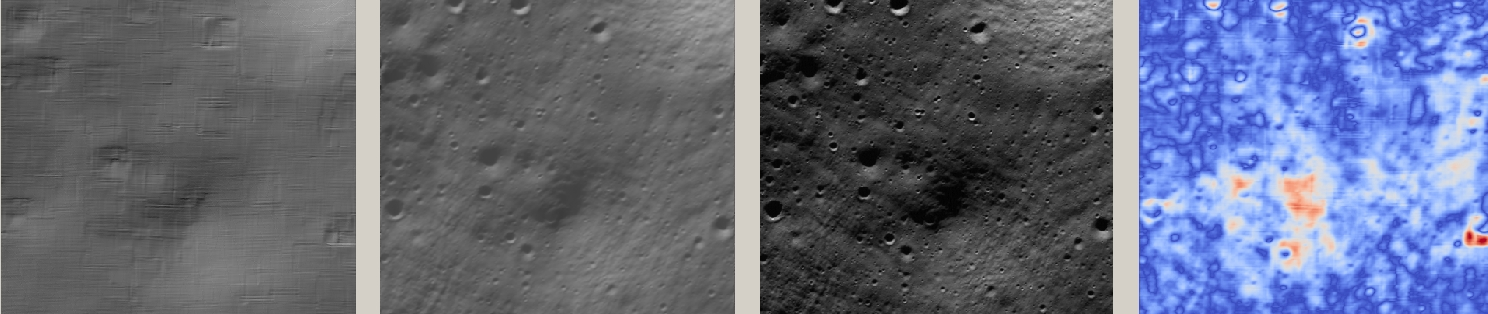
\includegraphics[width=7in]{images/sfs1.jpg}
\caption[sfs]{An illustration of \texttt{sfs}. The images are, from
  left to right, the original hill-shaded DEM, the hill-shaded DEM obtained
from \texttt{sfs}, the image A.cub map-projected onto the original DEM,
and the absolute difference of the original and final DEM, where the brightest
shade of red corresponds to a 2 meter height difference.}
\label{fig:sfs1}
\end{center}
\end{figure}

It can be seen that the optimized DEM provides a wealth of detail and
looks quite similar to the input image. It also did not diverge
significantly from the input DEM. We will see in the next section that
SfS is in fact able to make the refined DEM more accurate than the
initial guess (as compared to some known ground truth), though that is
not guaranteed, and most likely did not happen here where just one image
was used.

\section{SfS with multiple images in the presence of shadows}

In this section we will run \texttt{sfs} with multiple images. We would
like to be able to see if SfS improves the accuracy of the DEM rather
than just adding detail to it. We evaluate this using the following
(admittedly imperfect) approach. We resample the original images by a
factor of 10, run stereo with them, followed by SfS using the stereo
result as an initial guess and with the resampled images. As ground
truth, we create a DEM from the original images at 1 meter/pixel, which
we bring closer to the initial guess for SfS using
\texttt{pc\_align}. We would like to know if running SfS brings us even
closer to this ``ground truth'' DEM.

The most significant challenge in running SfS with multiple images is
that shape-from-shading is highly sensitive to errors in camera position
and orientation. The \texttt{sfs} tool can improve these by floating
them during optimization and by using a coarse-to-fine scheme, where
the problem is first solved using subsampled images and terrain then
it is successively refined.

If possible, it may still be desirable to bundle-adjust the cameras first
(section \ref{bundleadjust}). It is important to note that bundle adjustment may
fail if the images have sufficiently different illumination, as it will
not be able to find matches among images. In that case, it can be used
at least among the images forming the stereo pair that is used to create
the initial DEM, and one of these images should be specified as the
first input to SfS (as the tool keeps the camera pose of the first image
fixed while optimizing the poses of the other cameras to
it). Alternatively, \texttt{stereo\_gui} tool can be used to create the
matches manually (section \ref{stereo_gui}).

To make bundle adjustment and stereo faster, we first crop the images,
such as shown below (the crop parameters can be determined via
\texttt{stereo\_gui}).
\begin{verbatim}
  crop from = A.cub to = A_crop.cub sample = 1 line = 6644 nsamples = 2192 nlines = 4982
  crop from = B.cub to = B_crop.cub sample = 1 line = 7013 nsamples = 2531 nlines = 7337
  crop from = C.cub to = C_crop.cub sample = 1 line = 1 nsamples = 2531 nlines = 8305
  crop from = D.cub to = D_crop.cub sample = 1 line = 1 nsamples = 2531 nlines = 2740
\end{verbatim}
Then we bundle-adjust and run stereo
\begin{verbatim}
  bundle_adjust A_crop.cub B_crop.cub C_crop.cub D_crop.cub    \
    --min-matches 10 -o run_ba/run
  stereo A_crop.cub B_crop.cub run_full2/run --subpixel-mode 3 \
    --bundle-adjust-prefix run_ba/run
\end{verbatim}

This will result in a point cloud, \verb#run_full2/run-PC.tif#, which will
lead us to the ``ground truth'' DEM. As mentioned
before, we'll in fact run SfS with images subsampled by a factor of
10. Subsampling is done by running the ISIS \texttt{reduce} command
\begin{verbatim}
  reduce from = A_crop.cub to = A_crop_sub10.cub sscale = 10 lscale = 10
\end{verbatim}
and the same for the other images.

We run bundle adjustment and stereo with the subsampled images using
commands analogous to the above:
\begin{verbatim}
  bundle_adjust A_crop_sub10.cub B_crop_sub10.cub C_crop_sub10.cub D_crop_sub10.cub \
    --min-matches 1 -o run_ba_sub10/run --ip-per-tile 100000
 stereo A_crop_sub10.cub B_crop_sub10.cub run_sub10/run --subpixel-mode 3           \
   --bundle-adjust-prefix run_ba_sub10/run
\end{verbatim}
We'll obtain a point cloud named \verb#run_sub10/run-PC.tif#.

We'll bring the ``ground truth'' point cloud closer to the initial guess
for SfS using \texttt{pc\_align}:
\begin{verbatim}
  pc_align --max-displacement 200 run_full2/run-PC.tif run_sub10/run-PC.tif \
    -o run_full2/run --save-inv-transformed-reference-points
\end{verbatim}
This step is extremely important. Since we ran two bundle adjustment
steps, and both were without ground control points, the resulting clouds
may differ by a large translation, which we correct here. Hence we would like to 
make the ``ground truth'' terrain aligned with the datasets on which we 
will perform SfS. 

Next we create the ``ground truth'' DEM from the aligned high-resolution
point cloud, and crop it to a desired region:
\begin{verbatim}
  point2dem -r moon --tr 10 --stereographic --proj-lon 0 --proj-lat -90 \
    run_full2/run-trans_reference.tif
  gdal_translate -projwin -15540.7 151403 -14554.5 150473 \
    run_full2/run-trans_reference-DEM.tif run_full2/run-crop-DEM.tif
\end{verbatim}
We repeat the same steps for the initial guess for SfS:
\begin{verbatim}
  point2dem -r moon --tr 10 --stereographic --proj-lon 0 --proj-lat -90 \
    run_sub10/run-PC.tif
  gdal_translate -projwin -15540.7 151403 -14554.5 150473 \
    run_sub10/run-DEM.tif run_sub10/run-crop-DEM.tif
\end{verbatim}
Next we run \texttt{sfs} itself. Since our dataset has many shadows, we found
that specifying the shadow thresholds for the tool improves the
results. The thresholds can be determined using \texttt{stereo\_gui}.
\begin{verbatim}
  sfs -i run_sub10/run-crop-DEM.tif A_crop_sub10.cub C_crop_sub10.cub \
    D_crop_sub10.cub -o sfs/run --threads 1 --smoothness-weight 0.12  \
    --max-iterations 100 --reflectance-type 0 --float-exposure        \
    --float-cameras --use-approx-camera-models                        \
    --bundle-adjust-prefix run_ba_sub10/run                           \
    --shadow-thresholds "0.00162484 0.0012166 0.000781663"
\end{verbatim}
We compare the initial guess to \texttt{sfs} to the ``ground truth'' DEM
obtained earlier and the same for the final refined DEM using
\texttt{geodiff} as in the previous section. The mean error goes from
2.65 meters to 1.34 meters. Visually the refined DEM looks more detailed
as well as seen in figure \ref{fig:sfs2}.

We also show in this figure the first of the images used for SfS,
\verb#A_crop_sub10.cub#, map-projected upon the optimized DEM. Note that
we use the previously computed bundle-adjusted cameras when
map-projecting, otherwise the image will show as shifted from its true
location:
\begin{verbatim}
  mapproject sfs/run-DEM-iter28.tif A_crop_sub10.cub A_crop_sub10_map.tif \
    --bundle-adjust-prefix run_ba_sub10/run
\end{verbatim}
\begin{figure}[h!]
\begin{center}
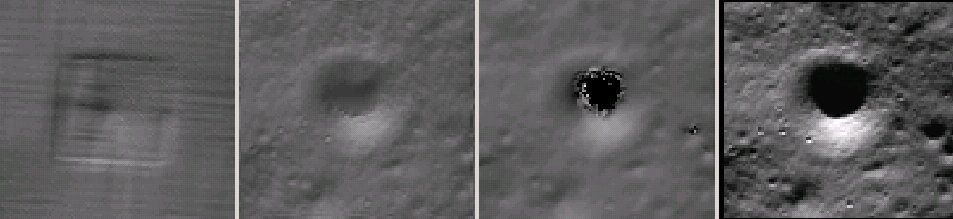
\includegraphics[width=7in]{images/sfs2.jpg}
\caption[sfs]{An illustration of \texttt{sfs}. The images are, from
  left to right, the hill-shaded initial guess DEM for SfS, the hill-shaded DEM obtained
from \texttt{sfs}, the ``ground truth'' DEM, and the first of the
images used in SfS map-projected onto the optimized DEM.}
\label{fig:sfs2}
\end{center}
\end{figure}

\section{Insights for getting the most of SfS}
\label{sfs:insights}

Here are a few suggestions we have found helpful when running \texttt{sfs}:

\begin{itemize}{}
\item First determine the appropriate smoothing term, by running a small clip, and using just one image.

\item Bundle-adjustment for multiple images is crucial. It is suggested to examine the measured intensity images output by \texttt{sfs} for some iterations using \texttt{stereo\_gui} with the options \texttt{-\/-single-window} and \texttt{-\/-use-georef} to see if the images overlay correctly, and if the overlay error appears to go down as the tool is running. If not, the cameras have a pose error that is too big for the algorithm to correct it.

\item If bundle adjustment is not successful, the option
\texttt{-\/--coarse-levels} is very helpful in fixing errors in camera
positions. It first runs SfS at a coarse resolution, and progressively
refines the results. A good value for the number of levels can be 3 to 5
(downsampling the images by a factor of 32 and 128 respectively), larger
values are suggested for larger camera errors.

\item Floating the albedo (option \texttt{-\/-float-albedo}) can introduce instability and divergence, it should be avoided unless albedo variation is seen in the images.

\item Floating the DEM at the boundary (option \texttt{-\/-float-dem-at-boundary}) is also suggested to be avoided.

\item Overall, the best strategy is to first use SfS for a single image and not float any variables except the DEM being optimized, and then gradually add images and float more variables and select whichever approach seems to give better results.
\end{itemize}
